\chapter{Ciclo de Vida}
\par O kit de automação desenvolvido pelo grupo apresenta um ciclo de vida que possui sua fase inicial de lançamento no mercado, crescimento, maturidade e declínio.

\begin{center}
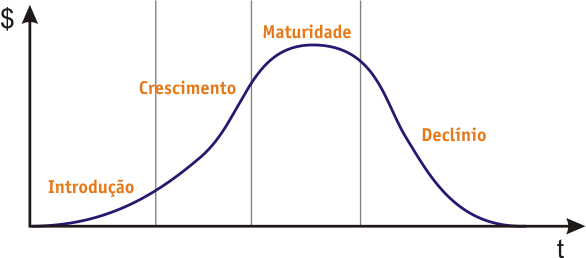
\includegraphics[width=\textwidth]{figuras/ciclodevida}
\end{center}

\par O público alvo do nosso kit são consumidores de classe média e de boa estabilidade financeira, como já foi citado. A ideia dele ser introduzido no mercado é por meio de prospecção passiva que é, basicamente, o cliente procurar nosso tipo de serviço e damos a ele as opções de pacote e fechamos com ele, ou seja, a interação cliente-produto vem de iniciativa do cliente.
\par Para atingir este público serão feitas divulgações em redes sociais e possíveis parcerias com comerciantes locais de imobiliárias e lojas de elétricas e eletrônicos para disponibilização dos equipamentos, além de um site da marca para divulgação.
\par Depois do produto instalado em algumas casas, toda a sua aceitação pelo mercado a partir daí será a base de como os clientes se adaptaram ao novo estilo de vida e qualidade do serviço oferecido pelo kit.
\par Como é algo inovador o serviço deve ser apresentado de forma singela e com uma qualidade que não deixe a desejar para que o produto final perpetue no mercado.
\par Com a adesão pelos consumidores, o kit deve ganhar maior divulgação e ampliação das vendas em possíveis lojas virtuais, em nosso próprio site e sites de vendas coletivas, para garantir clientes de diferentes localidades. Também deve ser montado uma equipe de suporte para analisar possíveis erros, falhas e melhorias que podem ser feitas para melhor eficiência e conforto para o usuário.
\par Ao garantirmos uma boa aceitação no mercado e grande número de vendas, deve-se trabalhar para manter a venda e os lucros altos, pois o preço de manutenção e resolução de problemas técnicos podem fazer o lucro total diminuir.
\par Um ponto importante a se perceber é quando o kit se torna obsoleto em relação aos concorrentes ou quando a tecnologia já está ultrapassada e, assim, é necessário criar atualizar o produto e manter a assistência técnica.
